\chapter{The Collatz Tree}

\section{The Connection between Groups and Graphs}
\label{sec:groups_graphs}
Let $(a_k)$ be a numerical sequence with $a_k=g^{(k)}(m)$, then a reversion produces an infinite number of sequences of reversely-written Collatz members \cite{Ref_Klisse_2010}.

Let $S$ be a set containing two elements $q$ and $r$, which are bijective functions over $\mathbb{Q}$:
\begin{equation}
\begin{array}{l}
q(x)=2x \\ 
r(x)=\frac{1}{3}(x-1)
\end{array}
\end{equation}

Let a binary operation be the right-to-left composition of functions $q\circ r$, where $q\circ r(x)=q(r(x))$. Composing functions is an associative operation. All compositions of the bijections $q$ and $r$ and their inverses $q^{-1}$ and $r^{-1}$ are again bijective. The set, whose elements are all these compositions, is closed under that operation. It forms a free group $F$ of rank 2 with respect to the free generating set $S$, where the group's binary operation $\circ$ is the function composition and the group's identity element is the identity function $id_{\mathbb{Q}}=e$. We call $e$ an \textit{empty string}. $F$ consists of all expressions (strings) that can be concatenated from the generators $q$ and $r$. The corresponding Cayley graph $Cay(F,S)=G$ is a regular tree whose vertices have four neighbors \cite[p.~66]{Ref_Loeh}. A tree is called \textit{regular} or \textit{homogeneous} when every vertex has the same degree, in this case, $d(v)=4$ for every vertex $v$ in $G$. The Cayley graph's set of vertices is $V(G)=F$, and its set of edges is $E(G)=\left\{\left\{f,f\circ s\right\}\mid f\in F,s\in\left(S\cup S^{-1}\right)\setminus\left\{e\right\}\right\}$ \cite[p.~57]{Ref_Loeh}. More precisely, the vertices are \textit{labeled} by the elements (strings) of $F$.

In conformance with graph-theoretical precepts \cite{Ref_Bondy_Murty},
\cite{Ref_Bonnington_Little}, \cite{Ref_Bender_Williamson}
we specify a subgraph $H$ of $G$ as a triple $\left(V(H),E(H),\psi_{H}\right)$ consisting of a set $V(H)$ of vertices, a set $E(H)$ of edges, and an incidence function $\psi_{H}$. The latter is, in our case, the restriction $\psi_{G}\vert_{E(H)}$ of the Cayley graph's incidence function to the set of edges that only join vertices, which are labeled by a string over alphabet $\{r,q\}$ without the inverses: $E(H)=\left\{\left\{f,f\circ s\right\}\mid f\in F,s\in S\setminus\left\{e
\right\}\right\}$.

This subgraph corresponds to the monoid $S^\ast$, which is freely generated by $S$ follows related thoughts \cite{Ref_Truemper_2014} that examine the Collatz problem in terms of a free semigroup on the set $S^{-1}$ of inverse generators. Note that this semigroup is not to be confused with an \textit{inverse semigroup} "in which every element has a unique inverse" \cite[p.~26]{Ref_Almeida}, \cite[p.~22]{Ref_Loeh}.

Let $Y^X=\{f\mid f\text{ is a map }X\rightarrow Y\}$ be the set of functions, which in category theory is referred to as the \textit{exponential object} for any sets $X$, $Y$. The evaluation function $ev:Y^X\times X\to Y$ sends the pair $(f,x)$ to $f(x)$. For a detailed description of this concept, see \cite[p.~127]{Ref_Johnsonbaugh}, \cite[p.~155]{Ref_MacLane_Birkhoff}, \cite[p.~54]{Ref_Novak_etal} and \cite[p.~188]{Ref_Pellissier}. We define the evaluation function $ev_{S^\ast}:S^\ast\times\{1\}\rightarrow\mathbb{Q}$ that evaluates an element of $S^\ast$, id est a composition of $q$ and $r$, for the given input value $1$. Furthermore we define the corestriction ${ev^0_{S^\ast}}$ of $ev_{S^\ast}$ to $\mathbb{N}$. Since a corestricion of a function resricts the function's codomain \cite[p.~3]{Ref_Helemskii}, the function $ev^0_{S^\ast}$ operates on a subset $T\subset S^\ast$ that contains only those compositions of $q$ and $r$, which return a natural number when inputting the value $1$.

The set $T$ forms not a monoid under function composition, for example $ev_{S^\ast}(qrq^4,1)=10$ and $ev_{S^\ast}(rq^6,1)=21$, but the composition $qrq^4rq^6$ does not lie in $T$, because the evaluation $ev_{S^\ast}(qrq^4rq^6,1)$ yields a value outside the codomain $\mathbb{N}$. However, each element of this set labels a vertex of a tree $H_{T}\subset H$, which is a proper subtree of $H$.

Let $U\subset T$ be a subset of $T$, which does not contain a reduced word with two or more successive characters $r$. The corresponding tree $H_{U}\subset H_{T}$ reflects Collatz sequences as demonstrated in figure~\ref{fig:1}.

\begin{remark}
When talking about trees having a root ("rooted trees"), another important concept should be explained: the \textbf{depth of a vertex} in a tree is the length of the path from the root to this vertex \cite[p.~226]{Ref_Sedgewick_2011}. In other words, it is the vertex's distance (the number of edges in the path) from the root. The root node has a depth of zero. The \textbf{level of a vertex} is its depth plus one $level(v)=depth(v)+1$. The level of a tree's root is always one. The \textbf{height of a vertex} is the number of edges on the longest downward path from that vertex and a leaf. Any leaf node has a height of zero. The \textbf{height of a tree} is the height of its root, or equivalently, the depth of its deepest vertex \cite[p.~226]{Ref_Sedgewick_2011}. The \textbf{size of a tree} is its number of nodes. One has to be careful, because the literature provides varying definitions. According to Rosen \cite[p.~804]{Ref_Rosen} for example, the level of a vertex is the length of the path from the root to this vertex; and the height of a tree is the largest vertex level in this tree.
\end{remark}

% trim=left top right bottom
\begin{figure}
	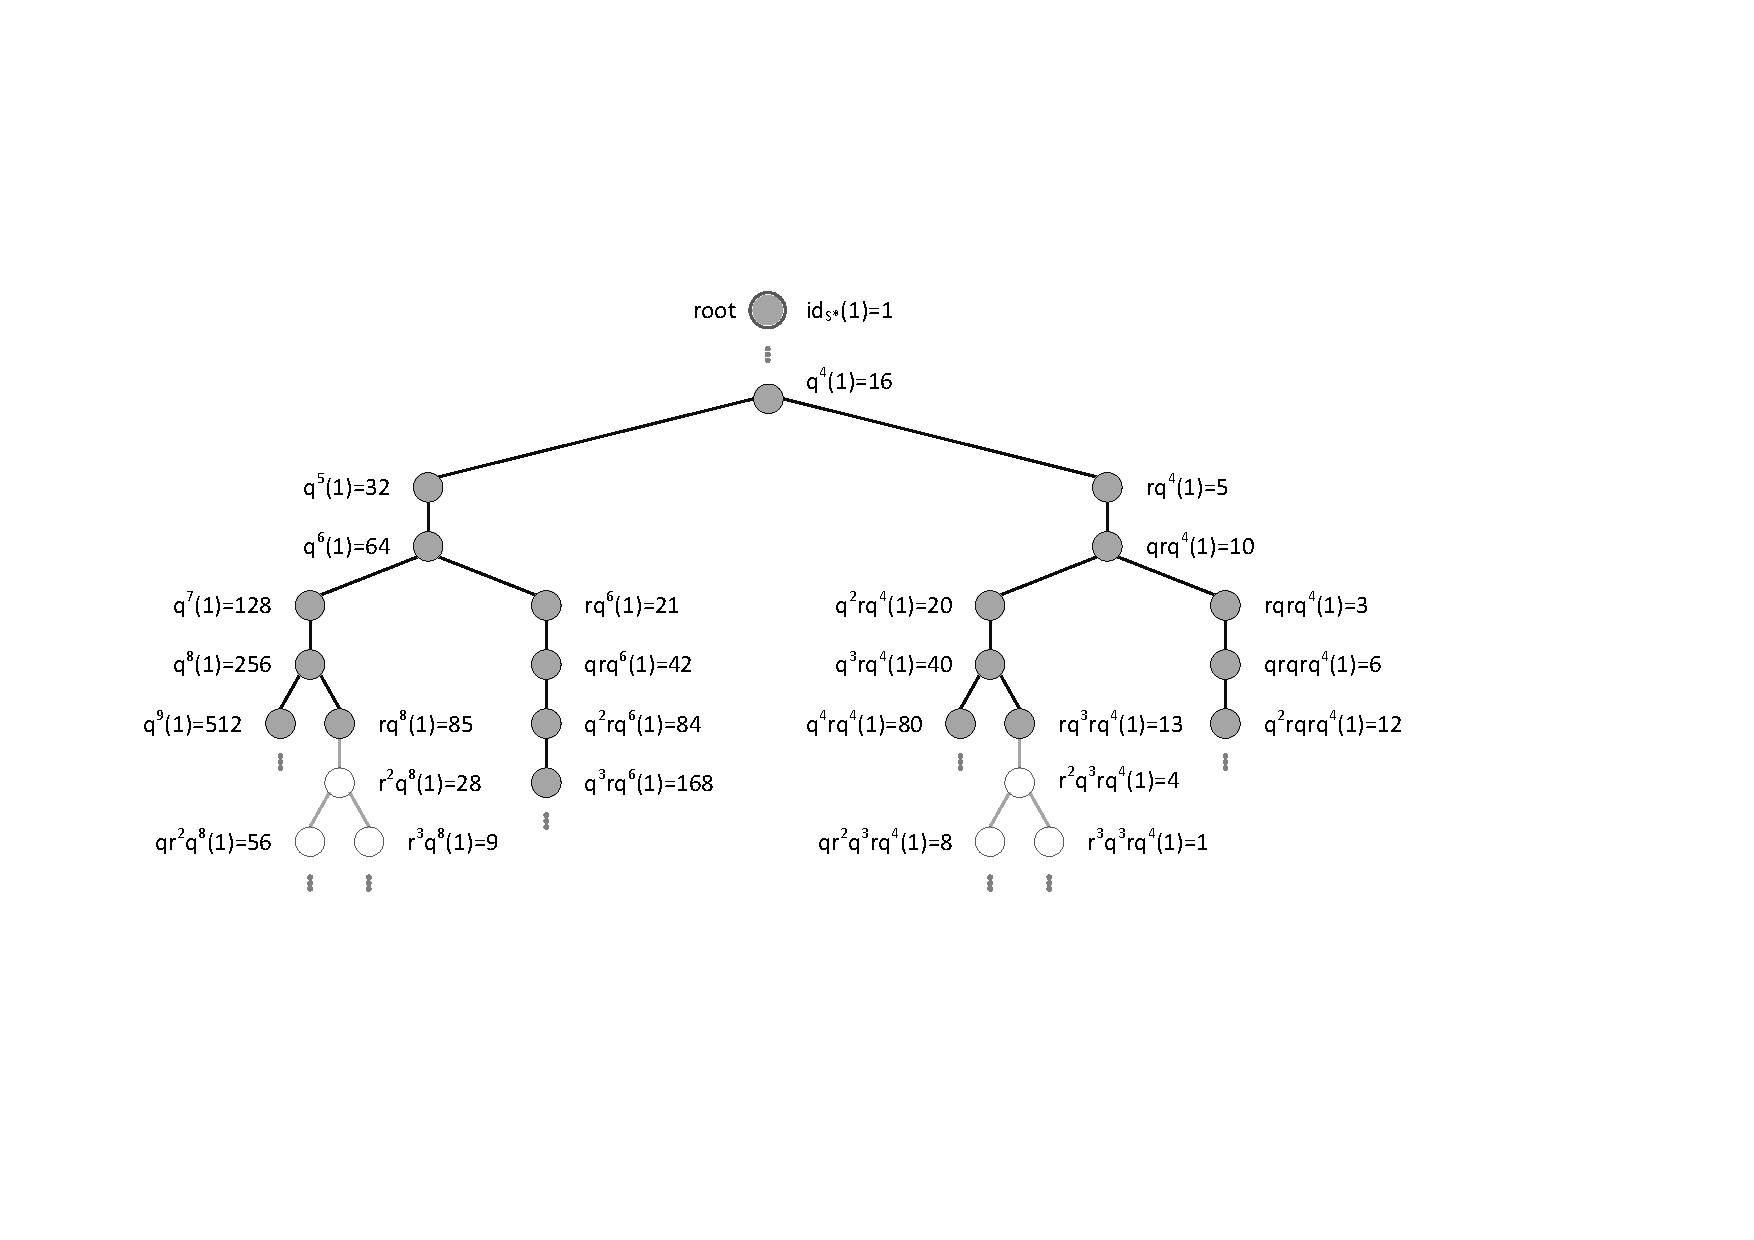
\includegraphics[trim=2.3cm 5.8cm 5.9cm 4.8cm, 
	width=1.00\textwidth,page=1]{figures/caytree.pdf}
	\caption{Small section of $H_T$ with darkly highlighted subtree $H_U$}
	\label{fig:1}
\end{figure}

\section{Defining the Tree}
The starting point for specifying our tree is $H_U$. Due to its significance, we first concertize $H_U$ by the definition~\ref{def:H_U} below, which establishes four essential characteristics.

\begin{definition}
The graph $H_U$ possess the following key properties:
\begin{itemize}
	\item \mbox{\boldmath$H_U$} \textbf{is a directed graph (digraph):} Fundamentally, when we consider the more general case, an undirected graph as a triple $(V,E,\psi)$, the incidence function maps an edge to an arbitary vertex pair $\psi : E\rightarrow\{X\subseteq V:\left|X\right|=2\}$. In a digraph, the set $V\times V$ represents ordered vertex pairs. Accordingly the incidence function is more specifically defined, namely as a mapping of the edges to that set $\psi : E\rightarrow\{(v,w)\in V\times V:v\neq w\}$, see \cite[p.~15]{Ref_Korte_Vygen}.
	\item \mbox{\boldmath$H_U$} \textbf{is a rooted tree:} According to Rosen \cite[p.~747]{Ref_Rosen}, a rooted tree is "a tree in which one vertex has been designated as the root and every edge is directed away from the root." Peculiarly, this definition considers the directionality as an inherent part of rooted trees. Unlike Mehlhorn and Sanders \cite[p.~52]{Ref_Mehlhorn_Sanders}, for example, who distinguish between an undirected and directed rooted tree.
	\par\smallskip
	\textit{Note: As long as we do not stipulate that vertices may collapse, it is absolutely guaranteed that the graph is a tree.}
	\item \mbox{\boldmath$H_U$} \textbf{is an out-tree:} There is exactly one	path from the root to every other node \cite[p.~52]{Ref_Mehlhorn_Sanders}, which means that edge directions go from parents to children \cite[p.~108]{Ref_Du_Ko_Hu}. This property is implied in Rosen's definition for a rooted tree as well by saying "every edge is directed away from the root." An out-tree is sometimes designated as \textit{out-arborescence} \cite[p.~108]{Ref_Du_Ko_Hu}.
	\item \mbox{\boldmath$H_U$} \textbf{is a labeled tree:} For defining a labeled graph, Ehrig et al. \cite[p.~23]{Ref_Ehrig_etal} use a label alphabet consisting of a vertex label set and an edge label set. Since we only label the vertices, in our case the specification of a vertex label set $L_V$ together with the vertex label function $l_V:V\rightarrow L_V$ is sufficient. Originally, we said vertex labels are strings over the alphabet $S=\{q,r\}$, through which the free monoid $S^\ast$ is generated. We illustrate labeling $H_U$ by defining $l_{V(H_U)}(v)=ev^0_{S^\ast}(l_{V(G)}(\iota(v)),1)$, whereby $\iota:V(H_U)\hookrightarrow V(G)$ is the inclusion map \cite[p.~142]{Ref_Childs} from the set of vertices of $H_U$ to the set of vertices from the previously defined Cayley graph $G$.
\end{itemize}
\label{def:H_U}
\end{definition}

We define a tree $H_{C,3}$ by taking the tree $H_U$ as a basis and for every vertex $v\in V(H_U)$ satisfying $2\mid l_{V(H_U)}(v)$, we contract the incoming edge. We attach the label of the parent of $v$ to the new vertex, which results by replacing (merging) the two overlapping vertices that the contracted edge used to connect. Visually, we obtain $H_{C,3}$ by contracting all edges in $H_U$ that have an even-labeled target vertex, which (due to contraction) gets "merged into its parent." Edge contraction is occasionally referred to as \textit{collapsing an edge}. For more details and examples on edge contraction, one can see Voloshin \cite[p.~27]{Ref_Voloshin} and Loehr \cite{Ref_Loehr}.

The tree $H_{C,3}$ is well known as the so-called \textit{Syracuse tree}, see for example \cite{Ref_Kleinnijenhuis_2020a}, \cite{Ref_Aberkane_2017}, and \cite{Ref_Aberkane_2020}. It is a \textit{minor of $H_U$}, since it can be obtained from $H_U$ "by a sequence of any vertex deletions, edge deletions and edge contractions" \cite[p.~32]{Ref_Voloshin}. The sequence of contracting the edges between adjacent (in our case even-labeled) vertices is called \textit{path contraction}.

A small section of the tree $H_{C,3}$, the Syracuse tree, is shown in figure~\ref{fig:2}. Other definitions of the same tree exist, see for example Conrow \cite{Ref_Conrow}, Bauer \cite[p.~379]{Ref_Bauer}, Batang \cite{Ref_Batang} or Jan Kleinnijenhuis and Alissa M. Kleinnijenhuis \cite{Ref_Kleinnijenhuis_2020a}, \cite{Ref_Kleinnijenhuis_2020b}.

\begin{figure}
	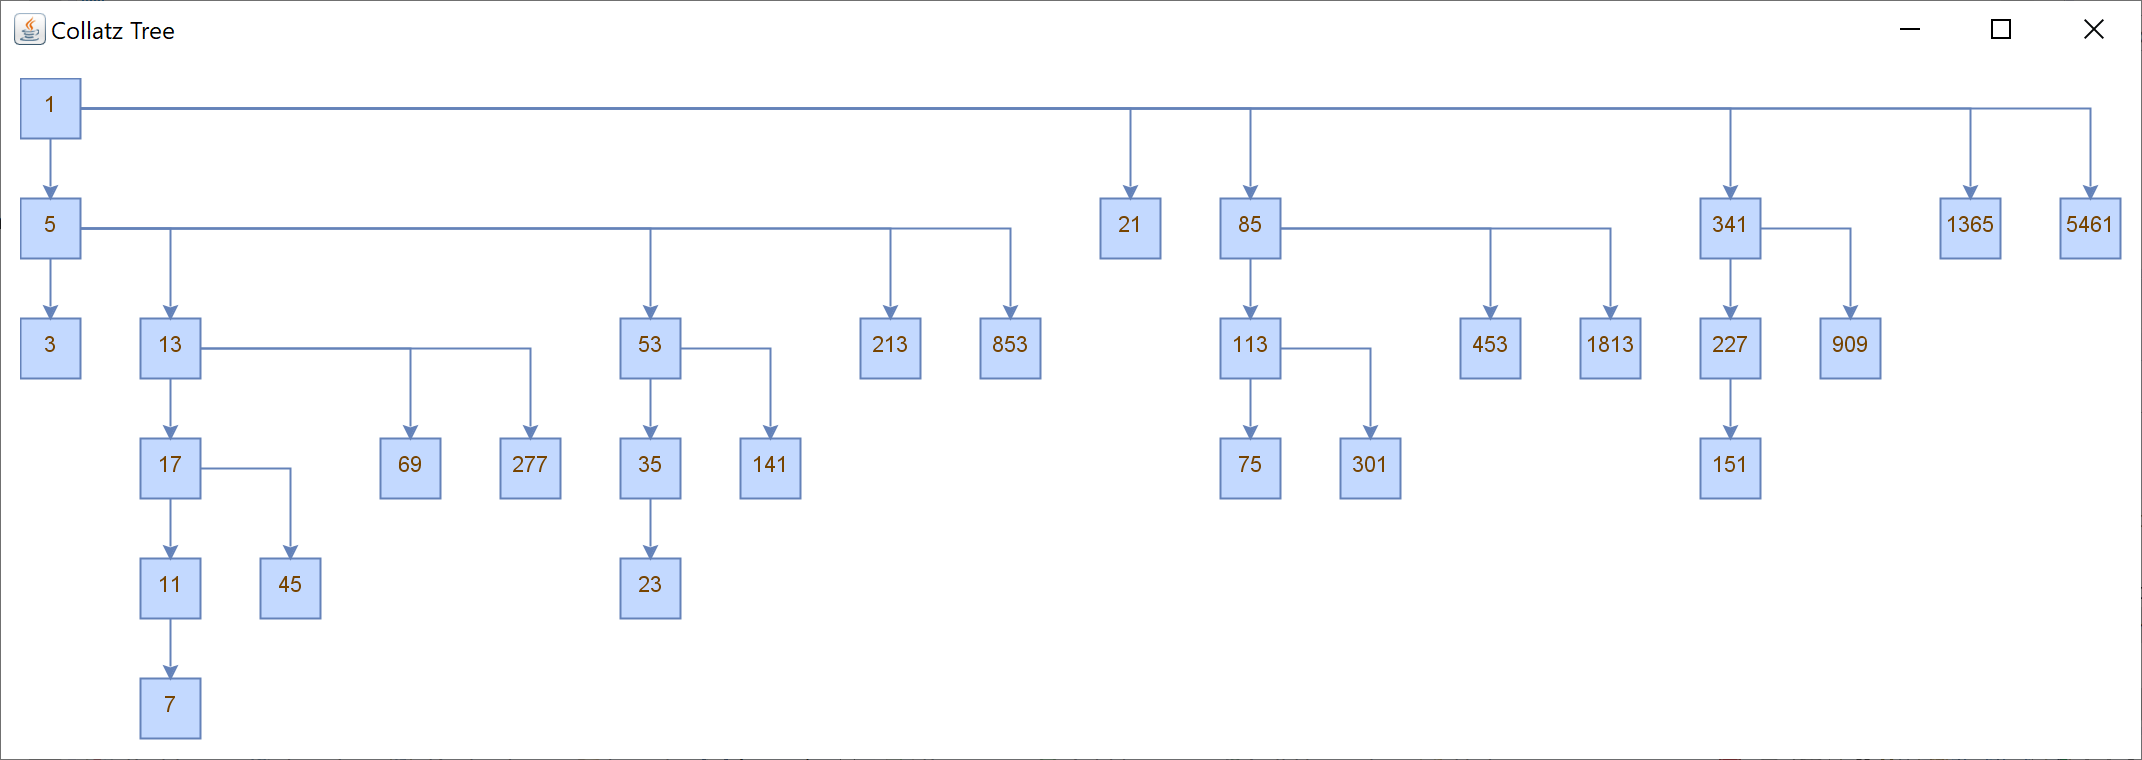
\includegraphics[width=1.00\textwidth]{figures/h_c3.png}
	\caption{Section of the Syracuse tree $H_{C,3}$ (displaying the trivial cycle is waived)}
	\label{fig:2}
\end{figure}

\section{\texorpdfstring{Relationship of successive nodes in $H_{C,3}$}{Relationship of successive nodes in HC3}}

Let $v_1$ and $v_{n+1}$ be two vertices of $H_{C,3}$, where $v_1$ is reachable from $v_{n+1}$ with $depth(v_1)-depth(v_{n+1})=n$. Hence, a path $(v_{n+1},\ldots,v_1)$ exists between these two vertices. Theorem~\ref{theo:1} specifies the following relationship between $v_1$ and $v_{n+1}$, empirically identified by Koch \cite{Ref_Koch_Github}.

\begin{theorem}
	\label{theo:1}
	$l_{V(H_{C,3})}(v_{n+1})=3^nl_{V(H_{C,3})}(v_1)\prod_{i=1}^{n}\left(1+\frac{1}{3l_{V(H_{C,3})}(v_{i})}\right)2^{-\alpha_i}$.
	In order to simplify readability, we waive writing down the vertex label function and put it shortly:\\
	$v_{n+1}=3^nv_1\prod_{i=1}^{n}\left(1+\frac{1}{3v_{i}}\right)2^{-\alpha_i}$.
	The value $\alpha_i\in\mathbb{N}$ is the number of edges which have been contracted between $v_i$ and $v_{i+1}$ in $H_U$.
\end{theorem}

In order to demonstrate the construction produced by theorem~\ref{theo:1} in an illustrative fashion, example~\ref{ex:vertices} runs through a concrete path in $H_{C,3}$.

\begin{example}
	\label{ex:vertices}
	For example, the two vertices $v_1=45$ and $v_{1+3}=v_4=5$ are 
	connected
	via the path $(5,13,17,45)$, see figure~\ref{fig:2}. Furthermore, one
	can retrace in figure~\ref{fig:3} the uncontracted path between these
	two nodes within $H_U$. When applied to this example,
	theorem~\ref{theo:1} produces the following:	
	\begin{center}
		$5=v_{1+3}=3^3\cdot45\cdot\left(1+\frac{1}{3\cdot45}\right)\cdot2^{-3}
		\cdot\left(1+\frac{1}{3\cdot17}\right)\cdot2^{-2}
		\cdot\left(1+\frac{1}{3\cdot13}\right)\cdot2^{-3}$
	\end{center} 
\end{example}

\begin{proof}
	\label{proof:1}
	This relationship of successive nodes can simply be proven inductively. For the base case, we set $n=1$ and retrieve
	\begin{center}
		$v_{1+1}=3v_1\left(1+\frac{1}{3v_1}\right)2^{-\alpha_1}
		=\left(3v_1+1\right)2^{-\alpha_1}=v_2$
	\end{center}
	The path from $v_2$ to $v_1$ can conformly be expressed by a string $rq\cdots q$ of $S^\ast$, because of $v_1=r\circ q^{\alpha_1}\left(v_2\right)$. We set $n=n+1$ for the step case, which leads to
	\begin{equation*}
	\begin{array}{cl}
	v_{n+2} &
	=3^{n+1}v_1\prod_{i=1}^{n+1}\left(1+\frac{1}{3v_i}\right)2^{-\alpha_i}\\
	&
	=3^{n+1}v_1\left(1+\frac{1}{3v_{n+1}}\right)2^{-\alpha_{n+1}}\prod_{i=1}^{n}\left(1+\frac{1}{3v_i}\right)2^{-\alpha_i}\\
	&
	=3\left(1+\frac{1}{3v_{n+1}}\right)2^{-\alpha_{n+1}}3^nv_1\prod_{i=1}^{n}\left(1+\frac{1}{3v_i}\right)2^{-\alpha_i}\\
	&
	=3\left(1+\frac{1}{3v_{n+1}}\right)2^{-\alpha_{n+1}}v_{n+1}\\
	&
	=\left(3v_{n+1}+1\right)2^{-\alpha_{n+1}}
	\end{array}
	\end{equation*}
	In this case the path from $v_{n+2}$ to $v_{n+1}$ is conformly 
	expressable by a string $rq\cdots q$ of $S^\ast$ too, since
	$v_{n+1}=r\circ q^{\alpha_{n+1}}\left(v_{n+2}\right)$.
\end{proof}

Even though the tree may theoretically contain two or more identically labeled vertices, it is essential to emphasize that we only consider such paths $(v_{n+1},\ldots,v_1)$ whose vertices are all labeled differently. Later in section~\ref{sec:cycles}, we even require that identically labeled nodes are one and the same. In order to correctly determine successive nodes using theorem~\ref{theo:1}, we must consider the halting conditions. These are specified in definition~\ref{def:halting_conditions}.

\begin{definition}
	\label{def:halting_conditions}
	When determining successive nodes starting at $v_1$ according to theorem~\ref{theo:1}, we halt if one of the following two conditions is fulfilled:
	\begin{enumerate}
		\item $v_{n+1}=1$
		\item $v_{n+1}\in\{v_1,v_2,\ldots,v_n\}$
	\end{enumerate}
	If the first condition applies, the Collatz conjecture is true for a specific sequence. When the second condition is fulfilled, the sequence has led to a cycle. For every starting node, except the root node (labeled with $1$), the Collatz conjecture is consequently falsified. Let us consider the example $v_1=13$, where the algorithm halts after two iterations, because the first condition is met:
	\[
	v_{n+1}=3^2\cdot\left(1+\frac{1}{3\cdot13}\right)\left(1+\frac{1}{3\cdot5}\right)\cdot2^{-7}=1
	\]
	
	If we examine the case $v_{1}=1$, we realize that the algorithm finishes after the first iteration, since both halting conditions are true. The sequence stops because the final node labeled with $1$ is reached. Furthermore, the sequence has led to a cycle:
	\[
	v_{n+1}=3\cdot\left(1+\frac{1}{3}\right)2^{-2}=1
	\]
	
	The trivial cycle is the only sequence where both conditions are fulfilled.
\end{definition}

\noindent
Theorem~\ref{theo:1} can be used for specifying the condition of a cycle as follows:

\begin{equation}
\label{eq:func_cycle}
\begin{array}{l}
v_{1}=3^nv_1\prod_{i=1}^{n}\left(1+\frac{1}{3v_i}\right)2^{-\alpha_i}
\\[\medskipamount]
2^{\alpha_1+\cdots+\alpha_n}=\prod_{i=1}^{n}\left(3+\frac{1}{v_i}\right)
\end{array}
\end{equation}

A similar condition has been formulated by Hercher \cite{Ref_Hercher} and Eric Roosendaal \cite{Ref_Roosendaal_2020}. Taking a first look at equation~\ref{eq:func_cycle}, we are able to recognize the trivial cycle for $n=1$. One might easily come to the false conclusion that the term only results in a natural number for this trivial cylce, since we are multiplying fractions. The following counterexample, starting at $v_1=31$, disproves this assumption:
\begin{equation*}
20480=\left(3+\frac{1}{31}\right)\left(3+\frac{1}{47}\right)
\left(3+\frac{1}{71}\right)\left(3+\frac{1}{107}\right)\left(3+\frac{1}{161}\right)\left(3+\frac{1}{121}\right)\left(3+\frac{1}{91}\right)\left(3+\frac{1}{137}\right)\left(3+\frac{1}{103}\right)
\end{equation*}

According to OESIS \cite{Ref_OESIS}, the integer $v_1=31$ is called \textit{self-contained}. The term self-contained is based on the fact that the node $v_{n+1}=v_{10}=155$ is divisible by the starting node $v_1=31$. Moreover, $v_{10}$ results from applying one and the same function (in this case the Collatz function) using $v_1$ as input, see also Guy \cite[p.~332]{Ref_Guy}. For such a case equation~\ref{eq:func_cycle} leads to a natural number, but not necessarily to a cycle. A cycle only occurs if the term results in a power of two. One example is the trivial cycle. We find another case when we choose the factor $5$ instead of $3$:
\begin{center}
	$128=2^7=\left(5+\frac{1}{13}\right)\left(5+\frac{1}{33}\right)
	\left(5+\frac{1}{83}\right)$
\end{center}

The above example shows that non-trivial cycles can be found if we generalize the Collatz conjecture by replacing the factor $3$ with the variable $k$. We study this generalized form and the occurance of cycles in section~\ref{sec:cycles}. A detailed elaboration of the divisibility and a deeper understanding of the tree $H_{C,3}$ needs to be performed in order to get towards any proof of the Collatz conjecture.

Generally, for any variant $kx+1$ it applies that if $v_1\mid v_{n+1}$, the product $\prod_{i=1}^n\left(k+\nicefrac{1}{v_i}\right)$ is natural.

\newpage

\begin{figure}[H]
	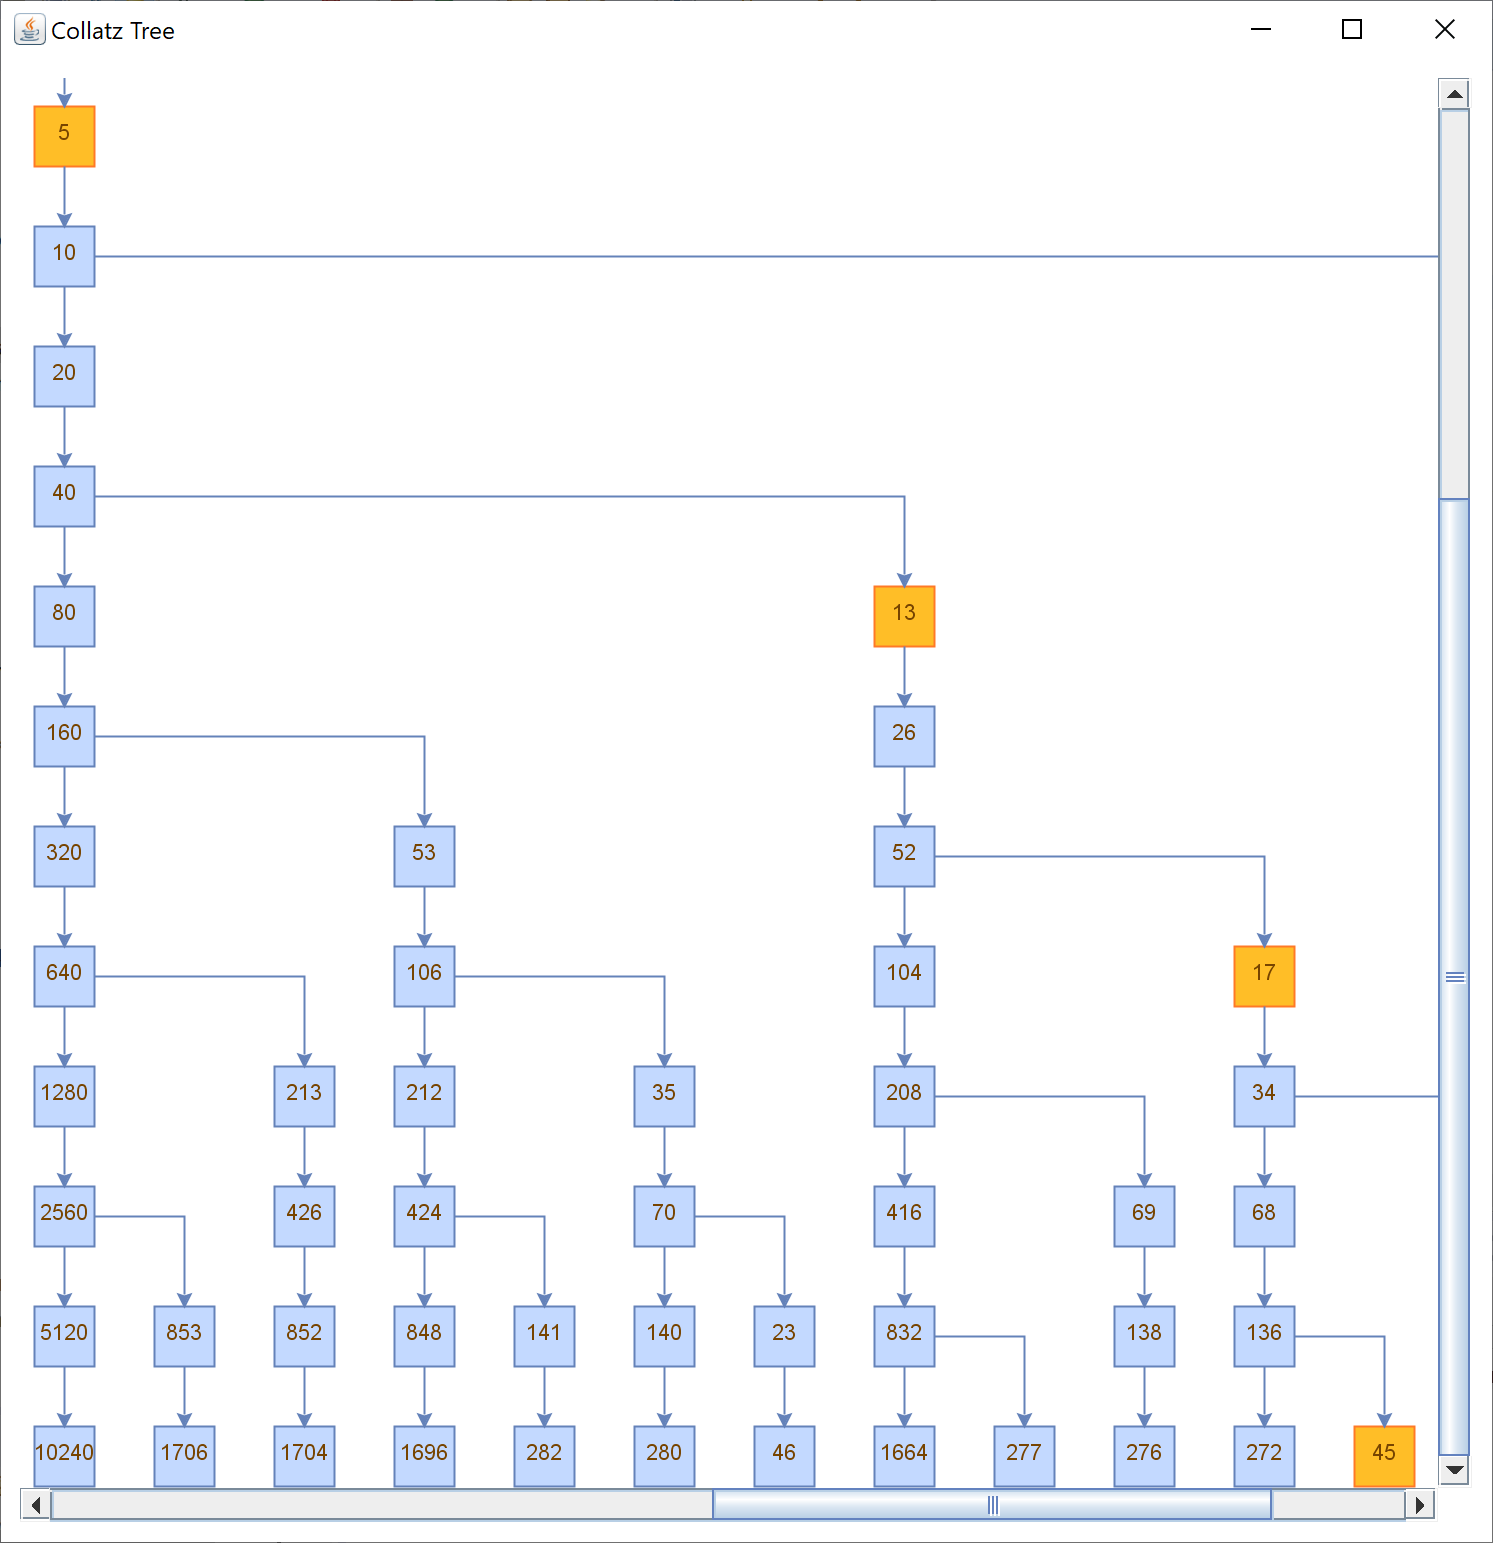
\includegraphics[width=1.00\textwidth]{figures/h_u.png}
	\caption{Section of $H_U$ containing the path from $5$ to $45$}
	\label{fig:3}
\end{figure}

\section{A note on the functions left-child and right-sibling}
Referring to the "left-child, right-sibling representation" of rooted trees \cite[p.~246]{Ref_Cormen_Leiserson_Rivest_Stein}, the function $\textit{left-child}:V\rightarrow V$ returns the leftmost child of a vertex $v$. Nesting this function $n$ times leads to the definition of a vertex's $n$-fold left-child, which is given by $\textit{left-child}^n(v)$. As shown in figure~\ref{fig:2}, for example $\textit{left-child}^3(13)=7$.

The function $\textit{right-sibling}:V\rightarrow V$ points to the sibling of a vertex $v$ immediately to its right \cite[p.~246]{Ref_Cormen_Leiserson_Rivest_Stein}. If this function is nested $n$ times, we get a vertex's $n$-fold right-sibling defined by $\textit{right-sibling}^n(v)$. One example is $\textit{right-sibling}^2(113)=1813$ which has been demonstrated in figure~\ref{fig:2} too.

\section{\texorpdfstring{Relationship of sibling nodes in $H_{C,3}$}{Relationship of sibling nodes in HC3}}
\label{sec:relationship_sibling_nodes_k3}

In a rooted tree, vertices which have the same parent are called "siblings" \cite[p.~702]{Ref_Johnsonbaugh}, \cite[p.~747]{Ref_Rosen}. Sibling vertices accordingly have the same depth and thus the same level.

Let $w$ be a vertex, from which a path exists to the vertex $v_1$. Let $v_2$ be the immediate right-sibling of $v_1$, then $l_{V\left(H_{C,3}\right)}\left(v_2\right)=4\cdot l_{V\left(H_{C,3}\right)}\left(v_1\right)+1$. This fact has been expressed differently by Kak \cite{Ref_Kak_2014} as follows: "If an odd number $a$ leads to another odd number (after several applications of the Collatz transformation) $b$, then $4a+1$ also leads to $b$."

Applied to our approach, consider $w$ as the parent of $v_1$ and $v_2$. Suppose, in $H_U$, a path consisting of $n+1$ edges goes from $w$ to $v_1$. Then we can straightforwardly show that $n$ edges in $H_U$ have been contracted between both nodes $w$ and $v_1$ and $n+2$ edges between $w$ and $v_2$ (for simplicity we again omit writing the label function):
\begin{equation}
\label{eq:next_sibling_k3}
\begin{array}{l}
		v_1=\frac{w\cdot2^n-1}{3}
		\\[\medskipamount]
		v_2=\frac{w\cdot2^{n+2}-1}{3}=4\cdot v_1+1
\end{array}
\end{equation}

For example, $n=3$ edges in $H_U$ have been contracted between $w=5$ and $v_1=13$ and $n+2=5$ edges between $w$ and $v_2=53$, whereby in $H_{C,3}$, the vertex $v_2$ is the right-sibling of $v_1$ and these two sibling vertices are immediate children of $w$.

Batang \cite{Ref_Batang} demonstrated that using the geometric series $s_n=1+4+4^2+\ldots+4^{n-1}=\nicefrac{4^n-1}{3}$ we are able to calculate the sibling nodes directly (see \cite[p.~191-192]{Ref_Teschl_2013} for more details on geometric series). Let us consider the sibling nodes $5,21,85,341$. The first sibling of $5$ is calculated by $s_1+4^1\cdot5=21$, the second sibling is $s_2+4^2\cdot5=85$, and the third is $s_3+4^3\cdot5=341$.

The same principle applies to the siblings $13,53,213,853$. The first sibling of $13$ is calculated by $s_1+4^1\cdot13=53$, the next one is $s_2+4^2\cdot13=213$, and the third is $s_3+4^3\cdot13=853$.

\section{\texorpdfstring{A vertex's left-child, $n$-fold right-sibling in $H_{C,3}$}{A vertex's left-child, n-fold right-sibling in HC3}}
\label{sec:left_child_right_sibling_3}

Let $w$ be a vertex in $H_{C,3}$ and $v_0$ the left-child of $w$. Using Koch's data science approach \cite{Ref_Koch_Github}, we empirically we have found out, that the $n$-fold right-sibling of $v_0$ can be calculated as follows:
\begin{equation}
\label{eq:nfold_right_sibling_3}
	v_n=\textit{right-sibling}^n(v_0)=\frac{1}{3}\left(w\cdot2^{2n+\pi_3(w\bmod 3)}-1\right)
\end{equation}

Hereby the function $\pi_3$, which appears in the exponent, is the self-inverse permutation (involution):
\begin{equation}
\label{eq:pi_3}
	\pi_3=\left(\begin{array}{cc}
	1 & 2\\
	2 & 1
	\end{array}\right)
\end{equation}

We consider permutations of the set $\{1,2\}$ and not of $\{0,1,2\}$, due to the fact that $w\bmod 3$ cannot be zero. A node $w$ in $H_{C,3}$, which is labeled by an integer divisible by $3$ is a leaf; and therefore such node has no left-child, more specifically it has no children at all. When setting $n=0$, we trivially retrieve the vertex's $w$ left-child:
\begin{center}
	$v_0=\textit{left-child}(w)=\frac{1}{3}\left(w\cdot2^{\pi_3(w\bmod 3)}-1\right)$
\end{center}

\begin{example}
\label{ex:siblings}
Let us refer to figure~\ref{fig:2} again and pick out $w=5$. Then the	vertex's $w$ left-child is $v_0=3$ and the threefold right-sibling
$v_3=213$:

\begin{equation*}
\begin{array}{l}
	v_0=\frac{1}{3}\left(5\cdot2^{\pi_3(5\bmod 3)}-1\right)=3
	\\[\medskipamount]
	v_3=\frac{1}{3}\left(5\cdot2^{2\cdot3+\pi_3(5\bmod 3)}-1\right)=213
\end{array}
\end{equation*}
\end{example}

We will now explain the reasons that are underlying this behavior. Basically two integers $a$ and $b$ are congruent modulo $n$ if their difference $a-b$ is divisible by $n$ or, to put it differently, if $a$ and $b$ have the same remainder when divided by $n$ \cite[p.~15]{Ref_Wolfart_2011}, \cite[p.~44]{Ref_Forster_2015}, \cite[p.~19]{Ref_Mueller-Stach_2011}:
\begin{equation}
\label{eq:congruence}
n|(a-b)\rightarrow a\equiv b\pmod n
\end{equation}

In modular arithmetic we are allowed to interpret integers as names, or to be more specific as \textit{representatives}, for their equivalence class and therefore reduce (or expand) a congruence as follows:
\begin{equation}
\label{eq:congruence_reduction}
(a+n)\equiv b\pmod n\rightarrow a\equiv b\pmod n
\end{equation}

This means, that in modular arithmetic both operations -- addition and multiplication -- are independent from the choice of representatives in the residue classes \cite[p.~16]{Ref_Wolfart_2011}.

The residue class (also termed congruence class) of the integers for a modulus $n$ is the set $[a]_n=\{a+k\cdot n|k\in\mathbb{Z}\}$ and sometimes denoted by $\bar a_n$ or by $a+n\mathbb{Z}$, see \cite[p.~15]{Ref_Wolfart_2011}, \cite[p.~120]{Ref_Schubert_2009}, \cite[p.~25]{Ref_Mueller-Stach_2011}. Let us put all possible remainders that arise from the division modulo $n$ together into a new set -- the set of all residue classes $[a]_n$. This set is known as the ring of integers modulo $n$ and denoted by $\mathbb{Z}/n\mathbb{Z}=\{[a]_n|a\in\mathbb{Z}\}$ and trivially $\mathbb{Z}/0\mathbb{Z}=\mathbb{Z}$ and for all $n\ne0$ we have $\mathbb{Z}/n\mathbb{Z}=\{[0],[1],\ldots,[n-1]\}$, see \cite[p.~15]{Ref_Wolfart_2011}, \cite[p.~25]{Ref_Mueller-Stach_2011}, \cite[p.~81]{Ref_Teschl_2013}.

Now there is one more tool that we will make use of later, and that is the \textit{Congruence Power Rule (CPR)}. It states that we are allowed to raise both sides of an congruence to the $n$-th power \cite[p.~19]{Ref_Mueller-Stach_2011}, \cite[p.~117]{Ref_Benjamin_2009}:
\begin{equation}
\label{eq:congruence_power_rule}
a\equiv b\pmod n\rightarrow a^n\equiv b^n\pmod n
\end{equation}

Let $G$ be a group and $a\in G$. If there exist an integer $d>0$ with $a^d=e$, then the smallest such $d$ is called the \textit{order} of $a$, written $d=\ord(a)$ \cite[p.~35]{Ref_Wolfart_2011}, \cite[p.~50]{Ref_Forster_2015}, \cite[p.~240]{Ref_Modler_Kreh_2012}. If no such $d$ exists, we formally write $\ord(a)=\infty$. The number of elements of $G$ is called the \textit{order} of $G$, written $\ord(G)$ \cite[p.~26]{Ref_Wolfart_2011}, \cite[p.~50]{Ref_Forster_2015}.

Let $G$ be a group and $a\in G$ an element of $G$. We consider the set of all elements $a^n\in G$ with $n\in\mathbb{Z}$. Since $a^na^m=a^{n+m}=a^ma^n$ and $(a^n)^{-1}=a^{-n}$, this set forms an abelian subgroup $H_a$ of $G$. This subgroup $H_a$ is also written $<a>$ and called the subgroup of $G$ \textit{generated} by $a$ \cite[p.~50]{Ref_Forster_2015}. A group $G$ is called \textit{cyclic}, if an $a\in G$ exists so that $G$ consists only of powers of $a$ (with exponents in $\mathbb{Z}$), thus if $G=<a>$ \cite[p.~34]{Ref_Wolfart_2011}, \cite[p.~50]{Ref_Forster_2015}, \cite[p.~240]{Ref_Modler_Kreh_2012}. In this case $\ord(a)=\ord(G)$, id est the order of an element $a\in G$ is equal to the order of the cyclic subgroup $<a>$ \cite[p.~50]{Ref_Forster_2015}.

Let us consider the cyclic group $<a>=\{e,a,a^2,\ldots,a^{n-1}\}$ and an element $b\in<a>$. Now let us face the question "How do we find the unique integer $0\le j\le n-1$, such that $a^j=b$?" This integer $j$ is denoted by $j=log_ab$ and it is called the \textit{discrete logarithm} of $b$ \cite[p.~255-256]{Ref_Stinson_Paterson_2019}. To make it more clear that we are talking about the discrete logarithm we write $j=\dlog_ab$ or more specifically $j=\dlog_{a,k}b$ if we solve the congruence $a^j\equiv b\pmod k$ which means we solve the equation $a^j\bmod k=b$, see \cite{Ref_Jain_2011}.

The multiplicative group of integers modulo $n$, denoted as $(\mathbb{Z}/n\mathbb{Z})^\times$ or briefly as $\mathbb{Z}_n^\ast$ contains those elements from $\mathbb{Z}/n\mathbb{Z}$ whose representatives are coprime to $n$ \cite[p.~87]{Ref_Teschl_2013}:
\begin{equation}
\label{eq:multiplicative_group_mod_n}
Z_n^\ast=\{a\in\mathbb{Z}/n\mathbb{Z}|\gcd(a,n)=1\}
\end{equation}

This group $\mathbb{Z}_n^\ast$ is a finite abelian group, which contains only the elements from the ring $\mathbb{Z}/n\mathbb{Z}$ that are invertible with respect to multiplication -- the units of $\mathbb{Z}/n\mathbb{Z}$. Within the ring $\mathbb{Z}/n\mathbb{Z}$ an element $a$ is invertible exactly if there exists an element $b$ such that $a*b\equiv1\pmod n$. An element inverse to $a$ exists exactly if $\gcd(a,n)=1$.

The \textit{multiplicative order} $\ord(a)$ of an element $a\in\mathbb{Z}_n^\ast$ is the smallest natural exponent $d$ which satisfies $a^d=1$. In other words, for a positive integer $n$ we say that an integer $a$ has multiplicative order $d$ modulo $n$ if $a^d\equiv1\pmod n$ where again $d$ is the smallest possible exponent \cite[p.~76]{Ref_Hutz_2018}, \cite[p.~32]{Ref_Shoup_2008}. To indicate that the order of $a$ refers to the modulus $n$, it is also often written $d=\ord_n(a)$. Recall that $\gcd(a,n)=1$, since $a\in\mathbb{Z}_n^\ast$

But what about the order of an multiplicative group of integers modulo $n$? It is exactly given by \textit{Euler's totient function}, see \cite[p.~27]{Ref_Wolfart_2011}:
\begin{equation}
\label{eq:multiplicative_group_order}
\ord(\mathbb{Z}_n^\ast)=\phi(n)
\end{equation}

Euler's totient function $\phi(n)$ counts the positive integers up to a given integer $n$ that are coprime to $n$ \cite[p.~49]{Ref_Forster_2015}. The fact that equation~\ref{eq:multiplicative_group_order} is correct follows directly from the definition of $\phi(n)$ -- we include into $\mathbb{Z}_n^\ast$ exactly those integers (representatives) from $\mathbb{Z}/n\mathbb{Z}$ that are coprime to $n$.

\begin{remark}
The elements of the ring of integers modulo $n$ do not form a group with respect to multiplication, because the element $0$ can not be inverted. But also $\mathbb{Z}/n\mathbb{Z}\setminus\{0\}$ does not form a group for a composite $n$, since there are always products of elements $a\ne0,b\ne0$ with $a*b=0$, which means that the "closure" property is not given \cite{Ref_Schwalen_2014}.
\end{remark}

An important theorem related to Euler's totient function, which we will use at a later stage, is Euler's theorem. Euler's theorem states that for an integer $a\ge2$ coprime to the modulus $n$ the following congruence holds \cite[p.~37]{Ref_Mueller-Stach_2011}, \cite[p.~56]{Ref_Forster_2015}, \cite[p.~104]{Ref_Teschl_2013}:
\begin{equation}
\label{eq:eulers_theorem}
a^{\phi(n)}\equiv1\pmod n
\end{equation}

This means that given $<a>=\mathbb{Z}_n^\ast$, for any generator $a$ coprime to the modulus $n$ the congruence $a^{\phi(n)}\equiv1\pmod n$ becomes true, where again $\phi(n)$ is the order of $\mathbb{Z}_n^\ast$ and thus the order of $a$ (see \ref{eq:multiplicative_group_order}). If $\phi(n)\equiv2\pmod4$ then the group $\mathbb{Z}_n^\ast$ is cyclic. Consequently the multiplicative group of integers modulo $n$ is cyclic for $n\in\{1,2,4,p^j,2p^j\}$, where $p$ being an odd prime and $j\ge1$ \cite{Ref_Schwalen_2014}.

At this point it is appropriate that we explain the mapping (permutation) given by \ref{eq:pi_3} in more detail. A helpful tool that we can use as a point of departure is the multiplicative group of integers modulo $3$. The element $2$ is a generator $<2>=\{1,2\}=\mathbb{Z}_3^\ast$, since $2\equiv\boldsymbol{2}\pmod3$ and $2^2\equiv4\equiv\boldsymbol{1}\pmod3$. The order of $2$ is $2$, since $2^2\equiv1\pmod3$. Now we use the CPR given by \ref{eq:congruence_power_rule} and obtain $(2^2)^{n+1}\equiv1^{n+1}\pmod3$ and the following generic congruence:
\begin{equation}
\label{eq:congruence_k3}
2^j2^{2n+2-j}\equiv1\pmod3
\end{equation}

Setting $j=0,1$ leads to the following behavior, which explains the formula~\ref{eq:nfold_right_sibling_3} and the mapping~\ref{eq:pi_3}:
{\renewcommand{\arraystretch}{1.8}
\begin{table}[H]
	\centering
	\begin{tabular}{|L|L|L|L|L|}
		\hline
		\thead{\boldsymbol{j}} &
		\thead{\textbf{congruence}~\ref{eq:congruence_k3}} &
		\thead{\textbf{node}\ \boldsymbol{w}} &
		\thead{\textbf{setting}\ \boldsymbol{w}\ \textbf{as per}\ \ref{eq:congruence_reduction}} &
		\thead{\textbf{divisibility as per}\ \ref{eq:congruence}}\\
		\hline
		0
		& 1\cdot2^{2n+2}\equiv1
		& w\in[1]_3
		& \multirowcell{2}{w\cdot2^{2n+\pi_3(w\bmod3)}\equiv1}
		& \multirowcell{2}{3|(w\cdot2^{2n+\pi_3(w\bmod3)}-1)}
		\\ \cline{1-3}
		1
		& 2\cdot2^{2n+1}\equiv1
		& w\in[2]_3
		& 
		& 
		\\ \hline
	\end{tabular}
\end{table}}

\begin{remark}
If addition is the group operation, as it is the case for example with the additive group of integers modulo $3$, denoted as $(\mathbb{Z}/3\mathbb{Z},+)$ or as $(\mathbb{Z}_3,+)$, then for an element $a$ the term $a^n$ means add (and not multiply) $a$ to itself $n$ times. In this specific case the group contains three elements $\mathbb{Z}_3=\{0,1,2\}$ and the identity element is $e=0$. The element $2$ is a generator $<2>=\{0,1,2\}=\mathbb{Z}_3$, since $2\equiv\boldsymbol{2}\pmod3$ and $2+2\equiv4\equiv\boldsymbol{1}\pmod3$ and $2+2+2\equiv6\equiv\boldsymbol{0}\pmod3$. The order of $2$ is $3$, because $2^3\equiv0\pmod3$.
\end{remark}

\section{\texorpdfstring{A vertex's left-child, $n$-fold right-sibling in $H_{C,5}$}{A vertex's left-child, n-fold right-sibling in HC5}}
\label{sec:left_child_right_sibling_5}

In the following we take a look at the tree $H_{C,5}$ -- the $5x+1$ variant of $H_C$, elaborated by Koch \cite{Ref_Koch_Github} using Data Science too. We must note that it is not a tree and moreover that not all of its vertices are reachable from the root. We define the permutation $\pi_5$ as follows:
\begin{center}
\label{eq:pi_5}
    $\pi_5=\left(\begin{array}{cccc}
    	1 & 2 & 3 & 4\\
    	4 & 3 & 1 & 2
    \end{array}\right)$	
\end{center}

Next, by letting $w$ be a vertex in $H_{C,5}$ and $v_0$ the left-child of $w$
we obtain the $n$-fold right-sibling of $v_0$ by the function that
is slightly different to the one defined by \ref{eq:nfold_right_sibling_3}:
\begin{equation}
\label{eq:nfold_right_sibling_5}
    v_n=\textit{right-sibling}^n(v_0)=\frac{1}{5}\left(w\cdot2^{4n+\pi_5(w\bmod 5)}-1\right)
\end{equation}

Analogous to \ref{eq:pi_3} only permutations on the set without zero
\{1,2,3,4\} need to be considered, since $w\bmod 5$ cannot be zero.
Otherwise, if $w\equiv 0 (\bmod 5)$ which means that $w$ were labeled
by an integer divisible by 5, then the node $w$ has no successor in $H_{C,5}$.

\noindent
By setting $n=0$, the function (above given by \ref{eq:nfold_right_sibling_5}) returns the left child of $w$:
\begin{center}
	$v_0=\textit{left-child}(w)=\frac{1}{5}\left(w\cdot2^{\pi_5(w\bmod 5)}-1\right)$
\end{center}

Equation~\ref{eq:nfold_right_sibling_5} has been identified empirically as well and can be explained using the cyclic group $<2>=\{1,2,3,4\}=\mathbb{Z}_5^\ast$. First of all, it is obvious that $2$ generates this group, since $2\equiv\boldsymbol{2}\pmod5$ and $2^2\equiv\boldsymbol{4}\pmod5$ and $2^3\equiv8\equiv\boldsymbol{3}\pmod5$ and $2^4\equiv16\equiv\boldsymbol{1}\pmod5$. The order is $4$ and according to \ref{eq:eulers_theorem} and \ref{eq:multiplicative_group_order} we have $2^{\ord(\mathbb{Z}_5^\ast)}\equiv2^{\phi(5)}\equiv2^4\equiv1\pmod5$. Again we use the CPR given by \ref{eq:congruence_power_rule} and obtain $(2^4)^{n+1}\equiv1^{n+1}\pmod5$ and the following generic congruence:
\begin{equation}
\label{eq:congruence_k5}
2^j2^{4n+4-j}\equiv1\pmod5
\end{equation}

Setting $j=0,1,2,3$ leads to the following behavior, which explains the formula~\ref{eq:nfold_right_sibling_5} and the mapping~\ref{eq:pi_5}:
{\renewcommand{\arraystretch}{1.8}
\begin{table}[H]
	\centering
	\begin{tabular}{|L|L|L|L|L|}
		\hline
		\thead{\boldsymbol{j}} &
		\thead{\textbf{congruence}~\ref{eq:congruence_k5}} &
		\thead{\textbf{node}\ \boldsymbol{w}} &
		\thead{\textbf{setting}\ \boldsymbol{w}\ \textbf{as per}\ \ref{eq:congruence_reduction}} &
		\thead{\textbf{divisibility as per}\ \ref{eq:congruence}}\\
		\hline
		0
		& 1\cdot2^{4n+4}\equiv1
		& w\in[1]_5
		& \multirowcell{4}{w\cdot2^{4n+\pi_5(w\bmod5)}\equiv1}
		& \multirowcell{4}{5|(w\cdot2^{4n+\pi_5(w\bmod5)}-1)}
		\\ \cline{1-3}
		1
		& 2\cdot2^{4n+3}\equiv1
		& w\in[2]_5
		& 
		&
		\\ \cline{1-3}
		2
		& 4\cdot2^{4n+2}\equiv1
		& w\in[4]_5
		& 
		&
		\\ \cline{1-3}
		3
		& 8\cdot2^{4n+1}\equiv1
		& w\in[3]_5
		& 
		&
		\\ \hline
	\end{tabular}
\end{table}}

Figure~\ref{fig:4} illustrates a small section of $H_{C,5}$ starting at its root. The particularly interesting thing about the graph $H_{C,5}$ is that it contains three cycles, the trivial cycle starting from the root $1,3$ and two non-trivial cycles $43,17,27$ and $83,33,13$. To be precise, three cycles are known (as it will become apparent later in section~\ref{sec:non_trivial_cycles}), and on the basis of present knowledge it cannot be ruled out with any certainty that other cycles exist.

\begin{figure}[H]
	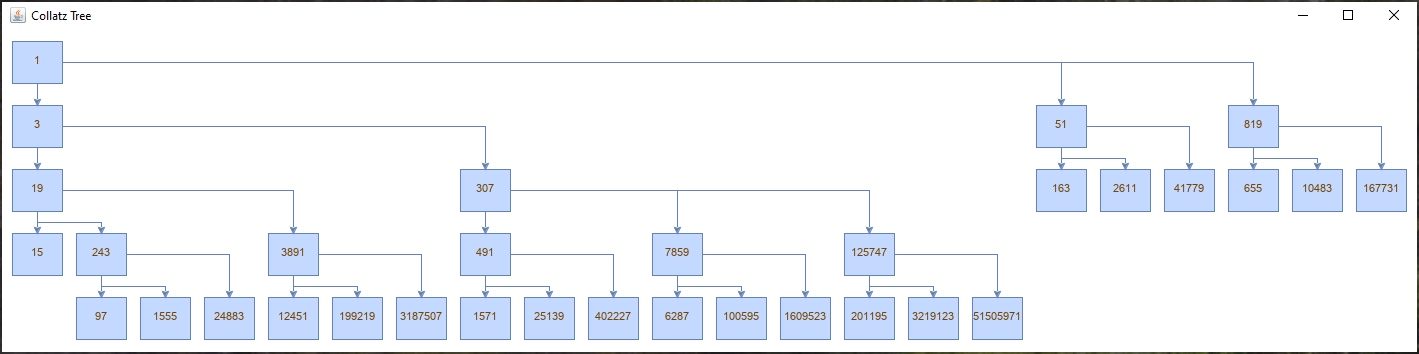
\includegraphics[width=1.00\textwidth]{figures/h_c5b.png}
	\caption{Section of the graph $H_{C,5}$ starting at its root (without branches that reflect a subsequence containing the trivial cycle)}
	\label{fig:4}
\end{figure}

\section{\texorpdfstring{A vertex's left-child, $n$-fold right-sibling in $H_{C,7}$}{A vertex's left-child, n-fold right-sibling in HC7}}
\label{sec:left_child_right_sibling_7}

Now we are able to develop the formula on our own that calculates for a given node $w$ the left-child and right-sibling in $H_{C,7}$. We refer to the cyclic group $\mathbb{Z}_7^\ast=\{1,2,3,4,5,6\}$. Note that in this case $2$ is not a generator of this group. But nevertheless $\mathbb{Z}_7^\ast$ is cyclic and $\ord(2)=3$ which gives $2^3\equiv1\pmod7$. Again we use the CPR given by \ref{eq:congruence_power_rule} and obtain $(2^3)^{n+1}\equiv1^{n+1}\pmod7$ and the following generic congruence:
\begin{equation}
\label{eq:congruence_k7}
2^j2^{3n+3-j}\equiv1\pmod7
\end{equation}

Setting $j=0,1,2$ leads to the following behavior, which produces the formula~\ref{eq:nfold_right_sibling_7} and the mapping~\ref{eq:pi_7}:
{\renewcommand{\arraystretch}{1.8}
\begin{table}[H]
	\centering
	\begin{tabular}{|L|L|L|L|L|}
		\hline
		\thead{\boldsymbol{j}} &
		\thead{\textbf{congruence}~\ref{eq:congruence_k7}} &
		\thead{\textbf{node}\ \boldsymbol{w}} &
		\thead{\textbf{setting}\ \boldsymbol{w}\ \textbf{as per}\ \ref{eq:congruence_reduction}} &
		\thead{\textbf{divisibility as per}\ \ref{eq:congruence}}\\
		\hline
		0
		& 1\cdot2^{3n+3}\equiv1
		& w\in[1]_7
		& \multirowcell{3}{w\cdot2^{3n+\pi_7(w\bmod7)}\equiv1}
		& \multirowcell{3}{7|(w\cdot2^{3n+\pi_7(w\bmod7)}-1)}
		\\ \cline{1-3}
		1
		& 2\cdot2^{3n+2}\equiv1
		& w\in[2]_7
		& 
		&
		\\ \cline{1-3}
		2
		& 4\cdot2^{3n+1}\equiv1
		& w\in[4]_7
		& 
		&
		\\ \hline
	\end{tabular}
\end{table}}

\begin{equation}
\label{eq:nfold_right_sibling_7}
v_n=\textit{right-sibling}^n(v_0)=\frac{1}{7}\left(w\cdot2^{3n+\pi_7(w\bmod 7)}-1\right)
\end{equation}

The mapping \ref{eq:pi_7} is not a permutation as in the case of $\pi_3$ and $\pi_5$, it is defined as follows:
\begin{equation}
\label{eq:pi_7}
\pi_7(n)=\begin{cases}
3	&	n=1\\
2	&	n=2\\
1   &   n=4
\end{cases}	
\end{equation}

\begin{figure}[H]
	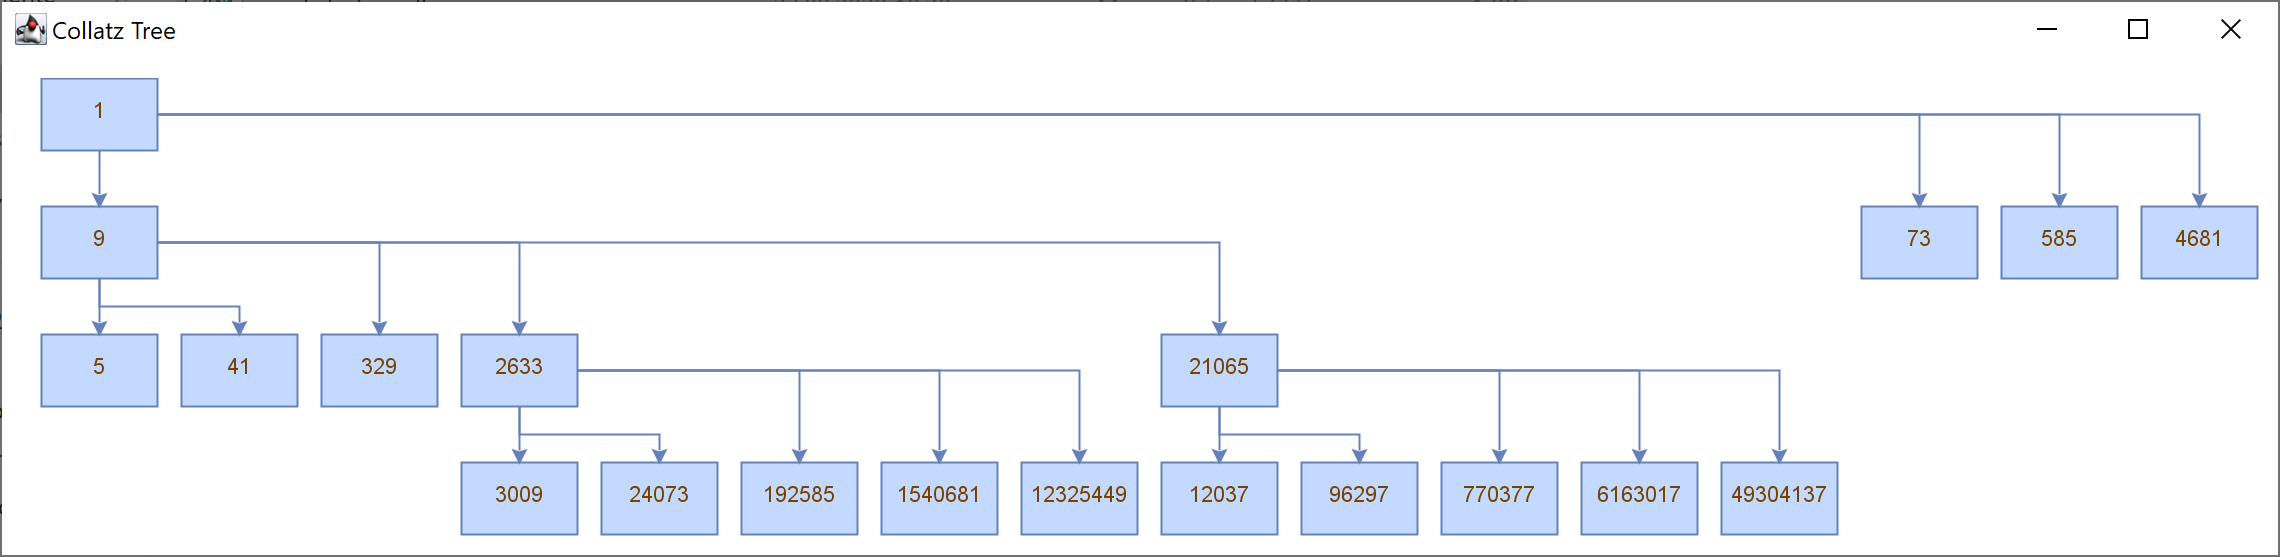
\includegraphics[width=1.00\textwidth]{figures/h_c7.png}
	\caption{Section of the graph $H_{C,7}$ starting at its root (without branches that reflect a subsequence containing the trivial cycle)}
	\label{fig:hc7}
\end{figure}

\section{\texorpdfstring{Generalizing the relationship of sibling nodes for $H_{C,k}$}{Generalizing the relationship of sibling nodes for HCk}}
In section~\ref{sec:relationship_sibling_nodes_k3} we have taken a closer look at the relationship of sibling nodes in $H_{C,3}$. But what is the formula for calculating the $n$-fold right-sibling of a given node $v_0$ generalized to the $kx+1$ variant of $H_C$? We remember that the multiplicative order $d=\ord_k(2)$ is the smallest natural exponent $d$ such that $2^d\equiv 1\pmod k$. In the case $k=3$ we can calculate the next sibling $v_1$ of a given node $v_0$ as follows: $v_1=v_0\cdot4+1$, see \ref{eq:next_sibling_k3}. Within $H_{C,7}$, the next sibling of $v_0$ is given by $v_1=v_0\cdot8+1$. In the case of $k=5$, we calculate the next sibling $v_1=v_0\cdot16+3$ and for $k=9$ we obtain the next sibling $v_1$ of a given node $v_0$ by $v_1=v_0\cdot64+7$. The general formula for calculating a given node's $v_0$ immediate right sibling is:
\begin{equation}
\label{eq:right_sibling_k}
v_1=v_0\cdot2^{\ord_k(2)}+\frac{1}{k}\left(2^{\ord_k(2)}-1\right)
\end{equation}

In order to calculate the $n$-fold right sibling of a given node $v_0$, we need to repeatedly nest $n$ times the (linear) function~\ref{eq:right_sibling_k}. For the sake of simplicity, let us substitute $a=2^{\ord_k(2)}$ and $b=\frac{1}{k}(2^{\ord_k(2)}-1)$. Then the $n$-fold right sibling of $v_0$ is obtained by the following structure:

\begin{flalign*}
v_n=\textit{right-sibling}^n(v_0)&=\left(\left(\left(v_0\cdot a+b\right)\cdot a+b\right)\cdot a+b\right)\cdots\\
&=v_0\cdot a^n+b(a^{n-1}+\ldots+a^2+a+1)=v_0\cdot a^n+b\frac{a^n-1}{a-1}
\end{flalign*}

Note that the term $b(a^{n-1}+\ldots+a^2+a+1)$ can be simplified using the $n$-th partial sum of a geometric series (\cite[p.~192]{Ref_Teschl_2013}). The resubstitution of both coefficients $a$ and $b$ leads us to the final generalized formula that calculates the $n$-fold right sibling of a node $v_0$ in $H_{C,k}$:
\begin{equation}
\label{eq:n_fold_right_sibling_k}
v_n=\textit{right-sibling}^n(v_0)=v_0\cdot2^{n\cdot\ord_k(2)}+\frac{1}{k}\left(2^{\ord_k(2)}-1\right)\cdot\frac{2^{n\cdot\ord_k(2)}-1}{2^{\ord_k(2)}-1}
\end{equation}

This can be verified by inserting $n=0$ and $n=1$ into formula~\ref{eq:left_child_n_fold_right_sibling_k} that calculates the a vertex's left-child, $n$-fold right-sibling of $H_{C,k}$:

\[\arraycolsep=1.6em
\begin{array}{ll}
v_0=\frac{1}{k}\left(w\cdot2^{\ord_k(2)-\dlog_{2,k}w}-1\right) & kv_0+1=w\cdot2^{\ord_k(2)-\dlog_{2,k}w}\\
v_1=\frac{1}{k}\left(w\cdot2^{2\ord_k(2)-\dlog_{2,k}w}-1\right) & kv_1+1=w\cdot2^{2\ord_k(2)-\dlog_{2,k}w}
\end{array}
\]

This brings us to the following quotient leading to the basic relationship between two sibling nodes that is given by equation~\ref{eq:right_sibling_k} in the form of $v_1=v_0\cdot a+b$:

\[
\frac{kv_1+1}{kv_0+1}=\frac{2^{2\ord_k(2)-\dlog_{2,k}w}}{2^{\ord_k(2)-\dlog_{2,k}w}}=2^{\ord_k(2)}
\]

Here we point out that the equation~\ref{eq:n_fold_right_sibling_k} of course only works for such $k$, where the order of two is not infinity $\ord_k(2)\ne\infty$. This means that, for instance, it does not work for $k=1$, id est for the $1x+1$ variant of $H_C$. However, this case is trivial and for the sake of completeness we have added a picture including some few words about $H_{C,1}$ in appendix~\ref{appx:x_plus_1_variant}.

\section{\texorpdfstring{Generalizing a vertex's left-child, $n$-fold right-sibling for $H_{C,k}$}{Generalizing vertex's left-child, n-fold right-sibling for HCk}}
In the following, we generalize the formulas, that has been developed in sections~\ref{sec:left_child_right_sibling_3}~-~\ref{sec:left_child_right_sibling_7} to calculate the left-child, $n$-fold right-sibling for a given node $w$ that is the direct parent node of $v_0$:
\begin{equation}
\label{eq:left_child_n_fold_right_sibling_k}
v_n=\textit{right-sibling}^n(v_0)=\frac{1}{k}\left(w\cdot2^{\ord_k(2)\cdot n+\ord_k(2)-\dlog_{2,k}w}-1\right)
\end{equation}

The discrete logarithm $\dlog_{2,k}w=j$ finds the smallest exponent $j$ such that $2^j\equiv w\pmod k$ respectively it solves the equation $2^j\bmod k=w$.
